\documentclass[tikz,border=15pt]{standalone}
\usepackage{tikz,amsmath,amssymb}
\usetikzlibrary{positioning,fit,shapes,arrows.meta,calc,backgrounds}

\definecolor{acaBlueLine}{HTML}{6080B0}     \definecolor{acaBlueFill}{HTML}{DBEAFE}
\definecolor{acaGreenLine}{HTML}{30A060}    \definecolor{acaGreenFill}{HTML}{A0D0A0}
\definecolor{acaOrangeLine}{HTML}{D06020}   \definecolor{acaOrangeFill}{HTML}{FFE6CC}
\definecolor{acaPurpleLine}{HTML}{6020D0}   \definecolor{acaPurpleFill}{HTML}{E1D5E7}
\definecolor{acaRedLine}{HTML}{B05050}      \definecolor{acaRedFill}{HTML}{F8CECC}
\definecolor{acaGreyLine}{HTML}{666666}     \definecolor{acaGreyFill}{HTML}{F5F5F5}
\definecolor{mambaGreen}{HTML}{059669}      \definecolor{mambaGreenFill}{HTML}{D1FAE5}

\begin{document}
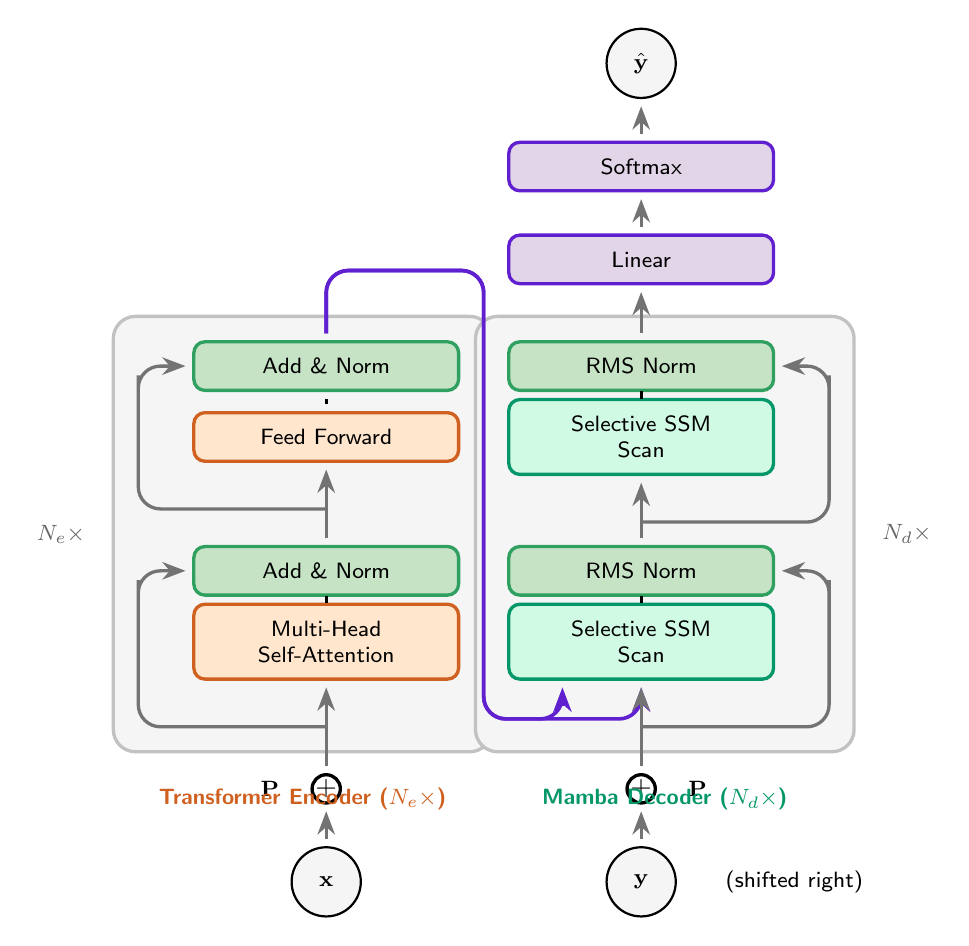
\begin{tikzpicture}[
    >=Stealth,very thick,
    arrow/.style={->,line width=1.2pt,black!55,rounded corners=8pt},
    block/.style={rectangle,fill=acaGreyFill,rounded corners=8pt,draw=acaGreyLine!40,very thick},
    layer/.style={rectangle,rounded corners=4pt,inner xsep=8pt,inner ysep=6pt,
        minimum height=1.6em,align=center,text width=2.8cm,draw,very thick,
        font=\footnotesize\sffamily,outer sep=3pt},
    layer_tf/.style={layer,fill=acaOrangeFill,draw=acaOrangeLine},
    layer_mm/.style={layer,fill=mambaGreenFill,draw=mambaGreen},
    layer_norm/.style={layer,fill=acaGreenFill!60,draw=acaGreenLine,minimum height=1.2em},
    layer_out/.style={layer,fill=acaPurpleFill,draw=acaPurpleLine},
    input/.style={circle,minimum width=2.5em,draw,fill=acaGreyFill,thick,
        font=\footnotesize\sffamily,outer sep=3pt},
]

% === INPUTS ===
\node[input] (src) at (1.25,-0.45) {$\mathbf{x}$};
\node[input] (tgt) at (5.25,-0.45) {$\mathbf{y}$};

% Positional encoding
\node[circle,draw,minimum size=0.3em,inner sep=0pt,above=1em of src,outer sep=3pt] (sum1) {$\mathbf{+}$};
\node[circle,draw,minimum size=0.3em,inner sep=0pt,above=1em of tgt,outer sep=3pt] (sum2) {$\mathbf{+}$};
\node[font=\footnotesize\sffamily,left=0.5em of sum1] {$\mathbf{P}$};
\node[font=\footnotesize\sffamily,right=0.5em of sum2] {$\mathbf{P}$};

% === TRANSFORMER ENCODER (left) ===
\node[layer_tf] (attn1) at (1.25,2.6) {Multi-Head\\Self-Attention};
\node[layer_norm] (norm1) at (1.25,3.5) {Add \& Norm};
\node[layer_tf] (ffn1)  at (1.25,5.2) {Feed Forward};
\node[layer_norm] (norm2) at (1.25,6.1) {Add \& Norm};
\draw[] (attn1) -- (norm1);
\draw[] (ffn1) -- (norm2);
\draw[arrow] (norm1) -- (ffn1);

% Encoder residual (curve around)
\draw[arrow] (attn1.south)++(0,-0.5) -| ($(norm1.west)+(-0.6,-0.4)$) |- (norm1.west);
\draw[arrow] (ffn1.south)++(0,-0.5) -| ($(norm2.west)+(-0.6,-0.4)$) |- (norm2.west);

% Encoder Nx wrap
\coordinate (e1) at ($(attn1.south east)+(0.2,-0.7)$);
\coordinate (e2) at ($(norm2.north west)+(-0.8,0.1)$);
\begin{scope}[on background layer]
    \node[block,fit=(e1)(e2)] (encoder) {};
\end{scope}
\node[font=\footnotesize\sffamily\bfseries,acaGreyLine,anchor=east] at ($(encoder.west)+(-0.2,0)$) {$N_e\times$};

% === MAMBA DECODER (right) ===
\node[layer_mm] (ssm1) at (5.25,2.6) {Selective SSM\\Scan};
\node[layer_norm] (norm3) at (5.25,3.5) {RMS Norm};
\node[layer_mm] (ssm2) at (5.25,5.2) {Selective SSM\\Scan};
\node[layer_norm] (norm4) at (5.25,6.1) {RMS Norm};
\draw[] (ssm1) -- (norm3);
\draw[] (ssm2) -- (norm4);
\draw[arrow] (norm3) -- (ssm2);

% Mamba residual
\draw[arrow] (ssm1.south)++(0,-0.5) -| ($(norm3.east)+(0.6,-0.4)$) |- (norm3.east);
\draw[arrow] (ssm2.south)++(0,-0.5) -| ($(norm4.east)+(0.6,-0.4)$) |- (norm4.east);

% Mamba Nx wrap
\coordinate (d1) at ($(ssm1.south east)+(0.8,-0.7)$);
\coordinate (d2) at ($(norm4.north west)+(-0.2,0.1)$);
\begin{scope}[on background layer]
    \node[block,fit=(d1)(d2)] (decoder) {};
\end{scope}
\node[font=\footnotesize\sffamily\bfseries,acaGreyLine,anchor=west] at ($(decoder.east)+(0.2,0)$) {$N_d\times$};

% === Cross-connection: Encoder → Mamba Decoder ===
\draw[arrow,acaPurpleLine,line width=1.3pt]
    (norm2.north) |- ($(norm2.north)+(1,0.8)$) -| ($(norm2.north)+(2,-1.5)$) |- ($(ssm1.south)+(-1,-0.4)$) -| ($(ssm1.south)+(-1,0)$);
\draw[arrow,acaPurpleLine,line width=1.3pt]
    (norm2.north) |- ($(norm2.north)+(1,0.8)$) -| ($(norm2.north)+(2,-1.5)$) |- ($(ssm1.south)+(0,-0.4)$) -| (ssm1.south);

% === OUTPUT ===
\node[layer_out,above=1.5em of norm4] (linear) {Linear};
\node[layer_out,above=1em of linear] (softmax) {Softmax};
\node[input,above=1em of softmax] (probs) {$\hat{\mathbf{y}}$};

\draw[arrow] (norm4) -- (linear);
\draw[arrow] (linear) -- (softmax);
\draw[arrow] (softmax) -- (probs);

% === MAIN FLOW ===
\draw[arrow] (src) -- (sum1);
\draw[arrow] (sum1) -- (attn1);
\draw[arrow] (tgt) -- (sum2);
\draw[arrow] (sum2) -- (ssm1);

\node[font=\footnotesize\sffamily] at ($(tgt.east)+(1.4,0)$) {(shifted right)};

% === HYBRID ANNOTATION ===
\node[font=\footnotesize\sffamily\bfseries,acaOrangeLine,anchor=north] at ($(encoder.south)+(0,-0.3)$)
    {Transformer Encoder ($N_e\times$)};
\node[font=\footnotesize\sffamily\bfseries,mambaGreen,anchor=north] at ($(decoder.south)+(0,-0.3)$)
    {Mamba Decoder ($N_d\times$)};

\end{tikzpicture}
\end{document}
